\documentclass[12pt]{article}
\usepackage[spanish,mexico]{babel}
	\selectlanguage{spanish}
\usepackage{graphicx}
\usepackage{amsmath}
\usepackage{wrapfig}
\usepackage{float}
\usepackage{hyperref}
\usepackage[utf8]{inputenc}


\title{Actividad 3: Efemérides}
\author{Ana Gabriela Carretas Talamante}
\date{04 de febrero de 2016}

\begin{document}
\maketitle
\section{Introducción}
En el estudio de los cuerpos celestes, una efemérides, es una tabla de valores que da las posiciones de los objetos astronómicos en el cielo en un momento o momentos dados \cite{W}. 

\begin{figure}[H]
\centering
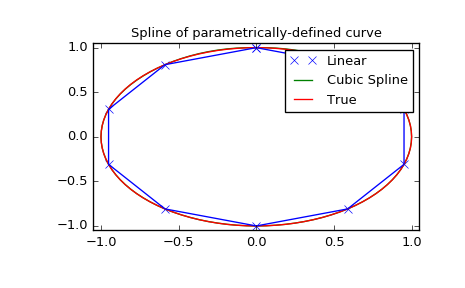
\includegraphics[width=7.5cm]{2}
\caption{Ejemplo de una interpolación para una curva parametrizada \cite{E}.}
\end{figure}

Para poder tener modelos matemáticos que describan el movimiento periódico de ciertos astros, se recurre a la utilización de interpolaciones con los datos arrojados por las efemérides. Interpolar se refiere a la obtención de nuevos puntos partiendo del conocimiento de un conjunto discreto de puntos \cite{I}. 

Hacer un programa que estime una función modelo para cierto fenómeno es la encomienda de la tercera actividad. Con respecto al programa base, se hicieron las modificaciones necesarias para poder obtener diferentes resultados.

\pagebreak

\subparagraph*{Programa original}
\begin{verbatim}
import numpy as np
import matplotlib.pyplot as plt
from scipy.interpolate import interp1d

# Original "data set" --- 21 random numbers between 0 and 1.
x0 = np.linspace(-1,1,21)
y0 = np.random.random(21)

plt.plot(x0, y0, 'o', label='Data')

# Array with points in between those of the data set for interpolation.
x = np.linspace(-1,1,101)

# Available options for interp1d
options = ('linear', 'nearest', 'zero', 'slinear', 'quadratic', 'cubic', 10)

for o in options:
    f = interp1d(x0, y0, kind=o)    # interpolation function
    plt.plot(x, f(x), label=o)      # plot of interpolated data

plt.legend()
plt.show()
\end{verbatim}

\begin{figure}[H]
\centering
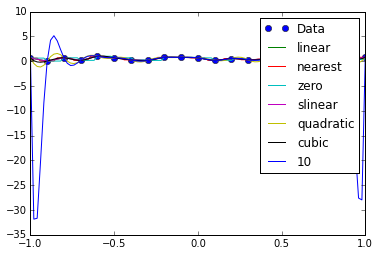
\includegraphics[width=7.5cm]{1}
\caption{Gráfica generada por el programa original.}
\end{figure}

\subparagraph*{10 puntos aleatorios con $x=[0,3]$ para la función $f(x)= \sin{2x}$.}
\begin{verbatim}
import numpy as np
import matplotlib.pyplot as plt
from scipy.interpolate import interp1d

# 10 números aleatorios entre 0 y 3.
xr = np.random.random(10)
x = xr*3
# "Data set" original
y = np.sin(3*x)

plt.plot(x, y, 'o', label='Data')

# Array con los puntos entre el "data set" original para la interpolación
xp = np.linspace(min(x), max(x), 10000)
# opciones para interp1d
options = ('linear', 'quadratic', 'cubic')
for o in options:
    f = interp1d(x, y, kind=o)    # función interpoladora
    plt.plot(xp, f(xp), label=o)      # gráfica de la función interpoladora
    
plt.legend(['data', 'linear', 'quadratic', 'cubic'], loc='best')
plt.show()
\end{verbatim}

\begin{figure}[H]
\centering
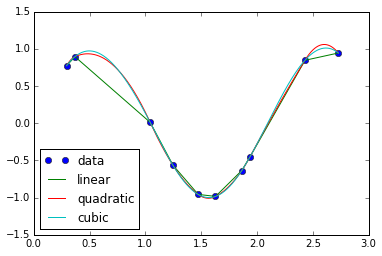
\includegraphics[width=7.5cm]{3}
\caption{Gráfica generada por el programa para la función $f(x)= \sin{2x}$.}
\end{figure}

\subparagraph*{20 puntos aleatorios con $x=[-10,10]$ para la función $f(x)= \displaystyle \frac{\sin{x}}{x}$.}
\begin{verbatim}
import numpy as np
import matplotlib.pyplot as plt
from scipy.interpolate import interp1d

# 20 números aleatorios entre -10 y 10.
xr = np.random.random(20)
x = (xr*20)-10
# "Data set" original
y = (np.sin(x))/x

plt.plot(x, y, 'o', label='Data')

# Array con los puntos entre el "data set" original para la interpolación
xp = np.linspace(min(x), max(x), 10000)
# opciones para interp1d
options = ('linear', 'quadratic', 'cubic')
for o in options:
    f = interp1d(x, y, kind=o)    # función interpoladora
    plt.plot(xp, f(xp), label=o)      # gráfica de la función interpoladora
    
plt.legend(['data', 'linear', 'quadratic', 'cubic'], loc='best')
plt.show()
\end{verbatim}

\begin{figure}[H]
\centering
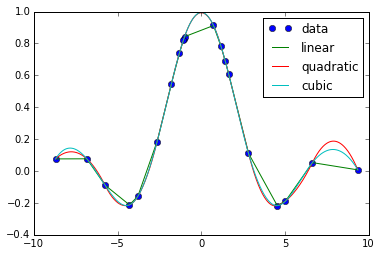
\includegraphics[width=7.5cm]{4}
\caption{Gráfica generada por el programa para la función $f(x)= \displaystyle \frac{\sin{x}}{x}$.}
\end{figure}

\subparagraph*{Dados 16 puntos aleatorios $x=[-3,3]$ para la función $f(x)= \displaystyle x^2\sin{2x}$.}
\begin{verbatim}
import numpy as np
import matplotlib.pyplot as plt
from scipy.interpolate import interp1d

# 16 números aleatorios entre -3 y 3.
xr = np.random.random(16)
x = (xr*6)-3
# "Data set" original
y = (x*x)*np.sin(2*x)

plt.plot(x, y, 'o', label='Data')

# Array con los puntos entre el "data set" original para la interpolación
xp = np.linspace(min(x), max(x), 10000)
# opciones para interp1d
options = ('linear', 'quadratic', 'cubic')
for o in options:
    f = interp1d(x, y, kind=o)    # función interpoladora
    plt.plot(xp, f(xp), label=o)      # gráfica de la función interpoladora
    
plt.legend(['data', 'linear', 'quadratic', 'cubic'], loc='best')
plt.show()
\end{verbatim}

\begin{figure}[H]
\centering
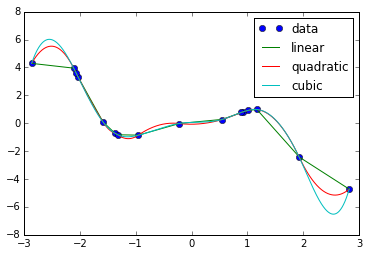
\includegraphics[width=7.5cm]{5}
\caption{Gráfica generada por el programa para la función $f(x)= \displaystyle x^2\sin{2x}$.}
\end{figure}

\subparagraph*{Dados 12 puntos aleatorios $x=[-2,2]$ para la función $f(x)= \displaystyle x^3\sin{3x}$.}
\begin{verbatim}
import numpy as np
import matplotlib.pyplot as plt
from scipy.interpolate import interp1d

# 12 números aleatorios entre -2 y 2.
xr = np.random.random(12)
x = (xr*4)-2
# "Data set" original
y = (x*x*x)*np.sin(3*x)

plt.plot(x, y, 'o', label='Data')

# Array con los puntos entre el "data set" original para la interpolación
xp = np.linspace(min(x), max(x), 10000)
# opciones para interp1d
options = ('linear', 'quadratic', 'cubic')
for o in options:
    f = interp1d(x, y, kind=o)    # función interpoladora
    plt.plot(xp, f(xp), label=o)      # gráfica de la función interpoladora
    
plt.legend(['data', 'linear', 'quadratic', 'cubic'], loc='best')
plt.show()
\end{verbatim}

\begin{figure}[H]
\centering
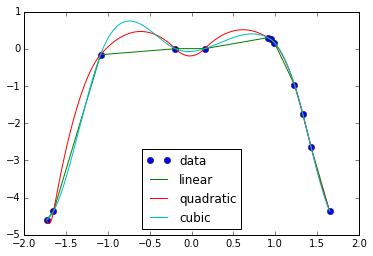
\includegraphics[width=7.5cm]{6}
\caption{Gráfica generada por el programa para la función $f(x)= \displaystyle x^3\sin{3x}$.}
\end{figure}

\begin{thebibliography}{6}

\bibitem{W}
Wikipedia,
\emph{Efemérides}. Recuperado el 02 de febrero de 2016 de \url{https://es.wikipedia.org/wiki/Efem\%C3\%A9rides}

\bibitem{I}
Wikipedia,
\emph{Interpolación}. Recuperado el 02 de febrero de 2016 de \url{https://es.wikipedia.org/wiki/Interpolaci\%C3\%B3n}

\bibitem{E}
Wikipedia,
\emph{Interpolation}. Recuperado el 02 de febrero de 2016 de \url{http://docs.scipy.org/doc/scipy/reference/tutorial/interpolate.html}

\bibitem{FC}
Lizárraga, C.
\emph{Actividad 3 (2016-1)}. Recuperado el 02 de febrero de 2016 de \url{http://computacional1.pbworks.com/w/page/104792695/Actividad\%203\%20\%282016-1\%29}

\end{thebibliography}

\end{document}
